
%% Mathematikumgebung
\usepackage{mathtools}
\usepackage{amssymb}  % Erweiterte Bibliothek mathematischer Symbole
\renewcommand{\epsilon}{\varepsilon}  % Nutze "richtiges" Epsilon

%% Grafikumgebungen
\usepackage{graphicx}  % Erweiterte Grafikumgebung
\usepackage{float}  % Automatische Positionierung von Bildern
\usepackage{floatflt}  % Grafiken im Text einbetten
\usepackage{subcaption}  %  Bildunterschriften fuer subfigures

%% Listenumgebung
\usepackage{enumerate}
\usepackage{textcomp}  % Korrekte serifenlose Aufzählungszeichen

%% Farbige Umrahmungen
%\usepackage{framed}
%\definecolor{shadecolor}{rgb}{0.9,0.9,0.9}

%% Chemische Formeln
\usepackage{chemfig}

%% Inhalt der Titelseite
\title{Advanced radiation and remote sensing}
\author{Stefan A Buehler, Lukas Kluft, Theresa Lang,\\ Christoph Sauter, Jakob Doerr, Laura Dietrich}
\date{\today}

%%%%%%%%%%%%%%%%%%%%%%%%%%%%%%%%%%%%%%%%%%%%%%%%%%%%%%%%%%%%%%%%%%%%%%
\begin{document}
\maketitle
\thispagestyle{empty}\pagestyle{empty}
\newpage
\tableofcontents
\newpage\pagestyle{fancy}



% CHAPTER 1 - INTRODUCTION
\section{Introduction}

This course is a continuation of the course \textit{radiation and
  remote sensing} in the bachelor program. Its goal is to
recapitulate the most important material of the previous course and to
give an extended knowledge on the physical processes involved like
spectroscopy, thermal radiation etc., in order to be able to work with
our radiative transfer model ARTS. After the course, you should have a
deeper understanding of radiation and remote sensing, and you should be
able to use ARTS and the tools around it for your own projects.

\subsection*{Contact}

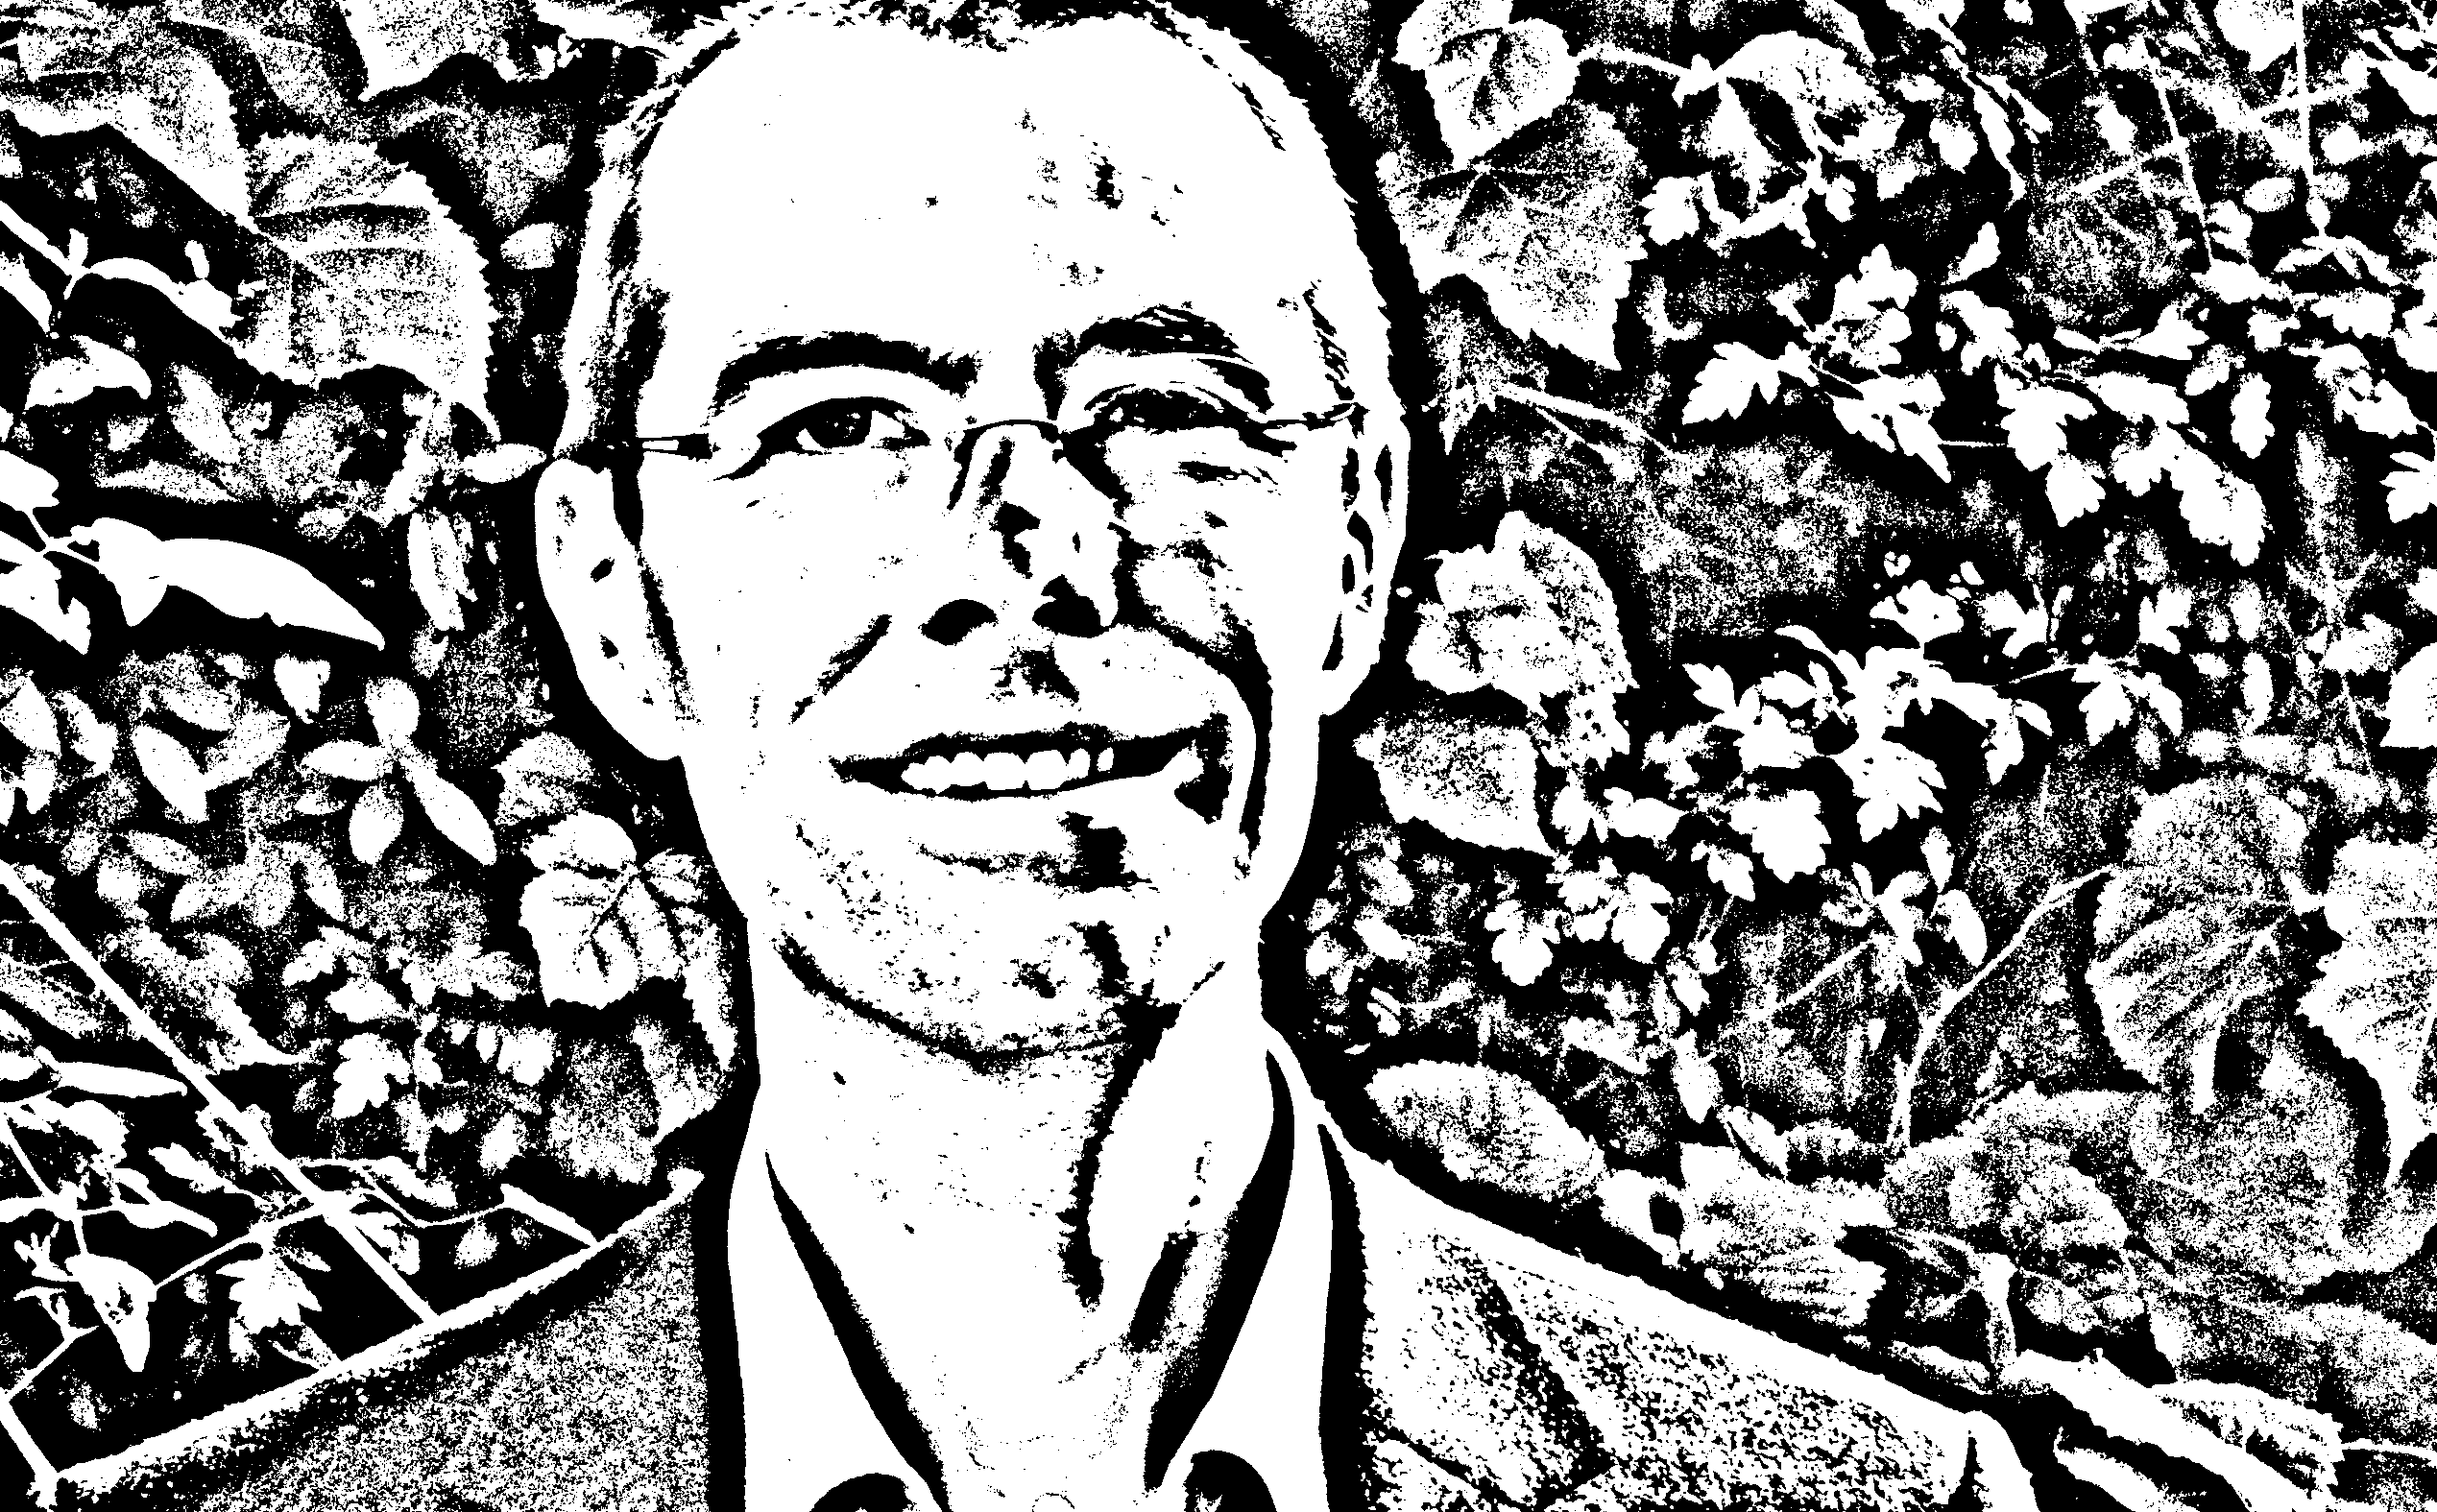
\includegraphics[width=4cm]{figures/buehler_portrait_sketch}
~
\begin{minipage}{0.5\linewidth}
  \vspace*{-1.6cm}
  Stefan A. Buehler\\
  Room 1534 (Geomatikum)\\
  Phone: +49 40 42838 8124\\
  Email: stefan.buehler(at)uni-hamburg.de\\
\end{minipage}

\subsection*{Modus operandi}

The course consists of a mixture of short lecture and a lot of
practical exercises. Don’t expect any polish. Don’t even expect
everything to work properly.

\subsection*{Examination}

As an exam, you are expected to investigate a small remote sensing or
radiation problem of your own choice. (Hopefully, you will find some
inspiration for a project during the course.) You have to present your
results in the last week of the course in a 10 minute
presentation. Presentations will be graded, and the grade will be
based on the criteria ambition level, originality, figure quality, and
presentation quality.

\subsection*{Contributions}

Many have contributed to this course: Theresa Mieslinger and Theresa
Lang prepared the initial exercises, based on my old exercises from a
course given at the University of Bremen, together with Björn-Martin
Sinnhuber. I have used some ideas from Björn-Martin's old course
notes, particularly in the area of rotational spectra.

The script is based on my handwritten notes from the first pass of the
course.  Lukas Kluft created the basic LaTeX structure and the initial
draft of Section \ref{sec:energy-states}. Theresa Lang created the
initial draft of Section \ref{sec:line_shape}. Christoph Sauter, Jakob
Doerr, and Laura Dietrich created initial drafts of other sections
from my notes.

\subsection*{Recommended reading}

Fundamentals of molecular spectroscopy by C.\ N.\
Banwell and E.\ M.\ McCash (Mc Graw Hill Verlag).


\section{Practical information}

This section can be also be found online on our webpage at
\url{https://www.mi.uni-hamburg.de/en/arbeitsgruppen/strahlung-und-fernerkundung/intern/howtos/arts-lecture.html}.

\subsection*{Getting started}

The material needed for the course is distributed via a subversion repository.
Subversion is a version control system and can be used via the command line
client \verb|svn|.

These steps have to be done only once:

\begin{verbatim}
cd ~
svn co https://arts.mi.uni-hamburg.de/svn/rt/arts-lectures/trunk arts-lectures
\end{verbatim}

\subsection*{Setting up the environment
(do this once in every new terminal)}
\label{sec:setup-env}


Every time you open a new terminal, you need to source the course environment.
If you know that your default shell (\verb|echo $SHELL|) is bash and not tcsh,
you can skip the first command:

\begin{verbatim}
bash --login
source ~/arts-lectures/bin/arts-init.bash
\end{verbatim}

You can check if the ARTS model is found by running:

\begin{verbatim}
arts --version
Updating the lecture package
\end{verbatim}

Use the \verb|svn update| command to ensure that you have the latest version
of the lecture files:

\begin{verbatim}
cd ~/arts-lectures
svn update
\end{verbatim}

\subsection*{Getting the lecture notes}

Change to the directory \texttt{script/} and run make:

\begin{verbatim}
cd ~/arts-lectures/script
make
\end{verbatim}

This will generate two PDF files, one optimised for viewing on the screen, one
optimised for printing.

\subsection*{Running the exercises}

Don't forget to run the \verb|source| command from the subsection
\hyperref[sec:setup-env]{`Setting up the environment'} above. You need to do
this every time you open a new terminal.

Change to the directory of the exercise and run arts for the exercise
controlfile. This example runs the first exercise:

\begin{verbatim}
cd ~/arts-lectures/exercises/01-rotational_spectra
arts absorption.arts
\end{verbatim}

This will run the ARTS program on the exercise controlfile. ARTS writes
several output files that can be found in the \texttt{results/} directory.

To plot the results you can use the Python script in the exercise directory,
which you can run by typing:

\begin{verbatim}
python plot_xsec.py
\end{verbatim}

This script will write the plots as PDF files in the \texttt{plots/}
subdirectory. You can use Evince to display the plots:

\begin{verbatim}
evince plots/plot_xsec_N2O_800hPa_300K.pdf
\end{verbatim}

\section{Absorption coefficients and absorption cross-sections}
\label{sec:absorption}

The law of Lambert, Beer, and Bouguer describes how radiation is
absorbed by a gas in a transmission experiment:
\begin{equation}
  dI(\nu)/ds = \alpha(\nu) I(\nu)\\
  I_1(\nu) = I_0(\nu) \exp \left( \int \alpha(\nu)ds \right)
\end{equation}
where $I$ is radiation intensity (in W/m$^2$/sr/Hz), $ds$ is distance in
the direction in which the radiation travels, $\alpha(\nu)$ is the
\emph{absorption coefficient} (in 1/m), and $\nu$ is frequency (in
Hz). We can take the above equations as the definition of $\alpha$.

For a gas, $\alpha(\nu)$ is richly structured; it contains
\emph{spectral lines} at certain frequencies where absorption is
strongly enhanced, and regions of little (or in any case less)
absorption in-between.

These lines come from quantum mechanics, to understand them we need to
understand the physical properties of single gas molecules. The
absorption coefficient $\alpha(\nu)$ can in good approximation be
decomposed as
\begin{equation}
  \alpha(\nu) = n \sigma(\nu)
\end{equation}
where $n$ is the number density (in 1/m$^3$) of the absorbing molecule
and $\sigma(\nu)$ is the \emph{absorption cross-section} (in
m$^2$). Cross-section on one hand refers to the unit, on the other
hand it allows also a simple geometrical interpretation of the
molecules as radiation-intercepting objects of a given cross-sectional
area. The linearity in the equation implies that the concentration of
the molecules is so low, that they do not `shadow' each other; twice
as many molecules means twice as much radiation absorbed. Earth's
atmosphere is so tenuous that this approximation is always valid. 

We can now turn to the physics underlying the absorption cross-section
$\sigma(\nu)$. 

\section{Energy states and photons}
\label{sec:energy-states}
Absorption and emission of a photon can happen if the internal energy of a
molecule changes. The difference in two energy states $E$ and the frequency of
the photon $\nu$ are connected through the Planck constant $h$.
\begin{equation}
  E_f - E_i = \Delta E = h \nu
\end{equation}
Figure \ref{fig:schematic_energies} is a graphical illustration of the
above equation.

The transitions between different energy levels can be divided into
three types, corresponding to different states of the molecule, as
show in Figure \ref{fig:transition_types}.  Each transition type is
characteristic for a specific region of the electro-magnetic spectrum.
One can distinguish changes in a molecules rotation (microwave),
vibration (infrared) and electronic transitions (UV/visible).

\begin{figure}
  \centering
  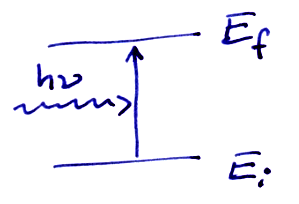
\includegraphics[width=5cm]{figures/schematic_energy_states}
  \caption{Schematic drawing of a molecular energy transition.}
  \label{fig:schematic_energies}
\end{figure}

\begin{figure}
  \centering
  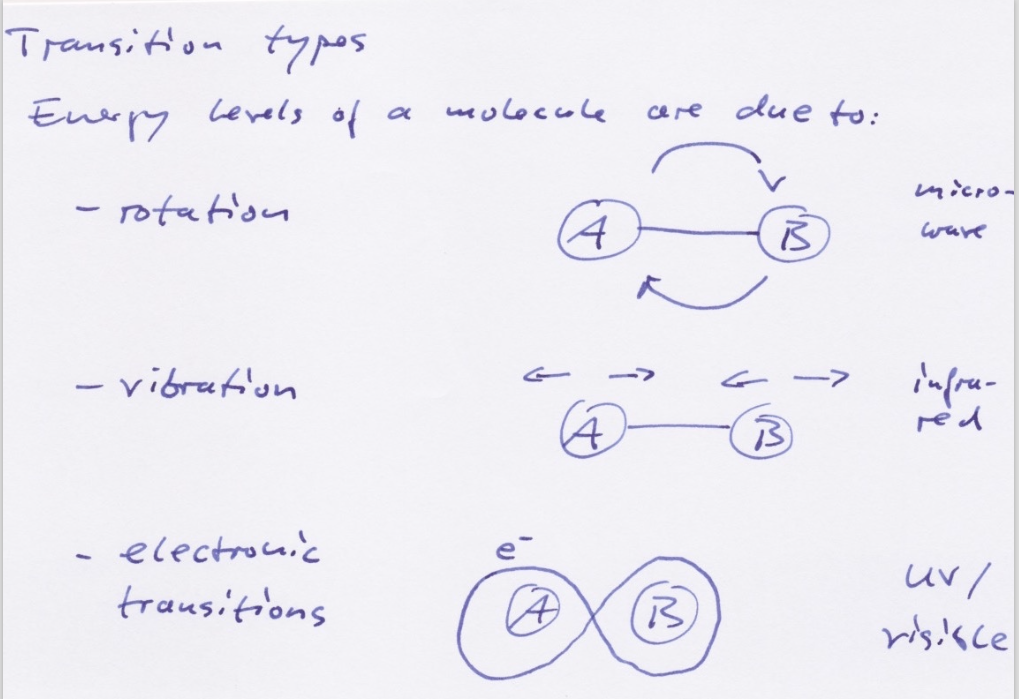
\includegraphics[width=\hsize]{figures/transition_types}
  \caption{Types of molecular energy transitions.}
  \label{fig:transition_types}
\end{figure}

Molecules consist of different atoms. There are diatomic molecules with two
atoms ($O_2$, $N_2$, $NO$, $HCl$, $CO$) and polyatomic molecules with
three or more atoms ($O_3$, $NO_2$, $CO_2$). We will mainly discuss
diatomic molecules, because they are easier to understand.

As shown in Figure \ref{fig:interaction_types}, one can distinguish
between three types of interaction between a photon and a molecule:
absorption, spontaneous emission and stimulated emission.

\begin{figure}
  \centering
  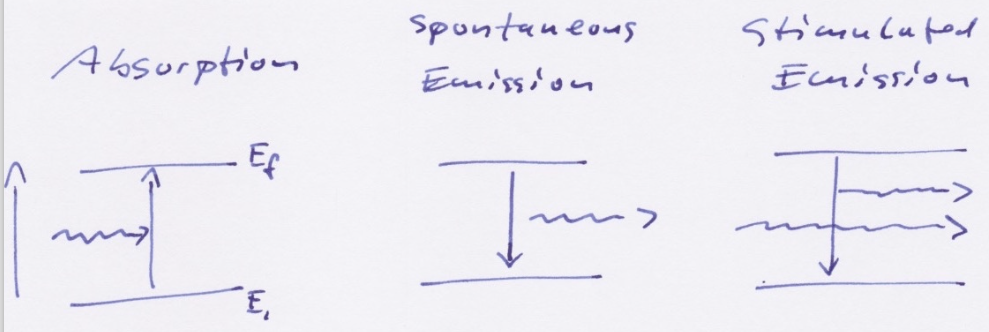
\includegraphics[width=\hsize]{figures/interaction_types}
  \caption{Ways for a molecule to interact with radiation.}
  \label{fig:interaction_types}
\end{figure}

There are three conditions to be fulfilled for a molecule to absorb a
photon:
\begin{enumerate}
\item The frequency of the photon has to match one of the molecule's energy
transitions.
\begin{equation}
  \Delta E = h \nu
\end{equation}

\item The net absorption has to be proportional to the difference of occupation
probabilities of states $i$ and $f$: $p_i - p_f$. Where $p_i$ is given by the
Boltzmann distribution (in local thermodynamic equilibrium).
\begin{equation}
  p_i = \frac{q_i e^{-E_i / (kT)}}
        {\sum_{j=1}^\infty q_j e^{-E_j / (kT)}}
\end{equation}
The denominator is often referred to as $Q(T)$. It has various names like total
internal partition sum, partition function, or Zustandssumme. The variable $q_i$
(or $q_j$) is called degeneracy factor. It is needed in order to take into account
that an energy level can exist more than once.

\item Absorption is proportional to the electric dipole matrix element $\mu_{if}$
between states $i$ and $f$.
\begin{equation}
  \mu_{if} = \mu \iiint \psi_f^*(x,y,z) \psi(x,y,z) \,dx\,dy\,dz
\end{equation}
Where $\mu$ is the magnitude of the dipole operator, $\mu_{if}$ is a constant
for each transition and $\psi$ is the wave function from quantum mechanics.
\end{enumerate}

Combining all conditions, one can define the absorption coefficient $\alpha$.
\begin{equation}
  \alpha(\nu) = n \sum_{f,i} S_{fi}(T) \delta(\nu_{fi} - \nu)
\end{equation}
With number density $n$, line strength $S_{fi}$, difference of state energies
$h\nu_{fi}$ and Dirac's delta function $\delta$ (physically not true, will be
replaced later by a so called "line shape" function.

The line strength is different for each transition and defined as follows.
\begin{equation}
    S_{fi} = \frac{8\pi^3\nu_{fi} \lvert\mu_{fi}\rvert^2 q_i}{3hcQ(T)}
      \left( e^{E_i/(kT)} - e^{E_f/(kT)} \right)
\end{equation}
Although this equation looks complicated, there is only one truly independent
variable, the temperature $T$. All other variables are constants of the
transition, or fundamental constants.

Spectral line catalogues are collections of these transition parameters. There
is one line in the catalogue for each spectral line (thousands for each
molecule). The most well-known is the HITRAN catalogue.


\section{Rotational spectra}
\label{sec:rotational_spectra}

\subsection{Moment of inertia and classical rotational energy}

The kinetic energy $E$ of a mass $m$ moving linearly at a speed $v$ is
\begin{equation}
  E = \frac{1}{2} m v^2 \quad .
\end{equation}
Using the definition of the momentum $p$ (\emph{German: Impuls})
\begin{equation}
  p = m v \quad ,
\end{equation}
this can also be written as
\begin{equation}
  E = \frac{p^2}{2m} \quad .
\end{equation}

Now imagine a mass that is not moving linearly, but \textbf{rotating},
as sketched in Figure \ref{fig:rotating_mass}. The formula for the
kinetic energy of a rotation looks very similar to the linear case:
\begin{equation}
  \label{eq:rotational_energy}
  E_r = \frac{1}{2} I \omega^2 = \frac{J^2}{2I} \quad ,  
\end{equation}
only velocity $v$ is replaced by the \textbf{angular velocity}
$\omega$ (\emph{German: Winkelgeschwindigkeit}), the mass $m$ is
replace by the \textbf{moment of inertia} $I$ (\emph{German:
  Trägheitsmoment}), and the momentum $p$ is replace by the
\textbf{angular momentum} $J$ (German: Drehimpuls).

\begin{figure}
  \centering
  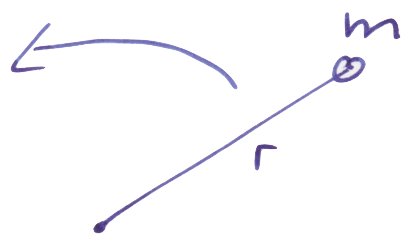
\includegraphics[width=0.4\textwidth]{figures/rotating_mass}
  \caption{Sketch of a rotating mass.}
  \label{fig:rotating_mass}
\end{figure}

These are defined as:
\begin{equation}
%  \label{eq:5}
  \omega = \frac{d\phi}{dt} \quad ,
\end{equation} 
where $\phi$ is the angle of rotation,
\begin{equation}
  \label{eq:def_I}
  I = m r^2 \quad ,
\end{equation}
where $r$ is the distance from the axis of rotation, and
\begin{equation}
  \label{eq:6}
  J = I \omega \quad .
\end{equation}

The moment of inertia $I$ is a measure of how `massive' an object
appears with respect to rotation.

\subsection{Using moments of inertia to classify molecules}

Any real object can not only rotate around a single axis, but could
rotate around any axis, and the moment of inertia $I$ depends on the
axis of rotation. We can describe any object by its three main axes of
rotation (the symmetry axes) and the associated three moments of
inertia $I_A$, $I_B$, $I_C$. (More exactly speaking, the inertia in
the general case is a 3x3 tensor, which becomes diagonal if the
coordinate system is aligned properly; the moments of inertia are the
eigenvalues of this tensor.)

We can use the moments of inertia to classify the molecules and divide
them into groups, as shown in Figure \ref{fig:molecule_types}.

\begin{figure}
  \centering
    \begin{tabular}{| c | c | c | c |}
      \hline
      Linear & Spherical top & Symmetric top & Asymmetric top \\
      \hline
             & & &  \\
      \chemfig{H-[,0.8]Cl} &
      \chemfig{C(-[:330]H)(-[:90,0.8]H)(-[:210]H)(-[:270,0.8]H)} &
      \chemfig{C(-[:0,0.8]F)(-[:140]H)(-[:180,0.8]H)(-[:220]H)} &
                                                                                                                                                      \chemfig{H-[:30,0.8]O-[:-30,0.8]H} \\
             & & & \\
             % \hline
      $I_A \approx 0$,   $I_B = I_C$ &
      $I_A = I_B = I_C$ &
      $I_A \neq 0$,   $I_B = I_C \neq I_A$ & 
      $I_A \neq I_B \neq I_C$ \\
      \hline
    \end{tabular}
  \caption{Using moments of inertia to classify molecules with
    different symmetry.}
  \label{fig:molecule_types}
\end{figure}

\subsection{Rotational energy for the special case of a diatomic molecule}

It is a good idea to first focus on the simplest type of molecule,
consisting of only two atoms. It can rotate around two axes, but has
the same moment of inertia for both.

Generalising Equation \ref{eq:def_I}, the total moment of inertia for
a collection of masses can be calculated as the sum of the moment of
inertia for each individual mass:
\begin{equation}
  I = \sum_i m_i r_i^2 \quad .
\end{equation}
We have to know the axis of rotation, so that we can calculate all the
$r_i$.

Per definition, the molecule will rotate around its \textbf{center of
  gravity}. (If the center of gravity would move, there would be a
translational motion of the entire molecule, but here we want to focus
on rotation as a internal degree of freedom of the molecule.) The
center of gravity has the property that
\begin{equation}
m_1 r_1 = m_2 r_2
\end{equation}

The geometry is as shown in Figure \ref{fig:reduced_mass}. It can
be shown, that this two-body problem can be reduced to an equivalent
one-body problem, the rotation of a single mass $\mu$ around an axis
at a distance $r_0$, which simply is given by
\begin{equation}
  r_0 = r_1 + r_2 \quad .
\end{equation}

\begin{figure}
\begin{center}
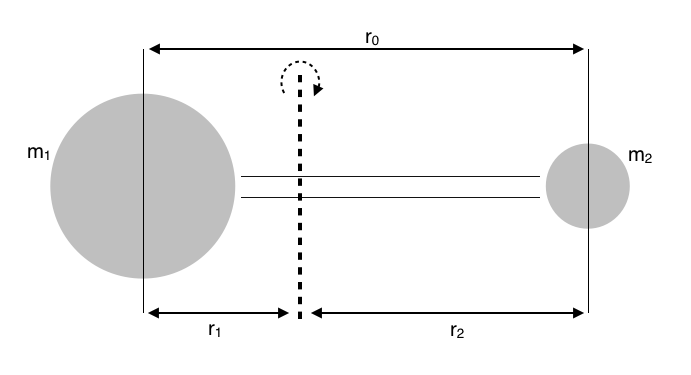
\includegraphics[width=1\textwidth]{figures/Reduced_mass}
\caption{Sketch of a diatomic and asymmetric molecule of atomic masses $m_1$ and $m_2$ at a distance of $r_0$.}
\label{fig:reduced_mass}
\end{center}
\end{figure}

The \textbf{reduced mass} $\mu$ is given by
\begin{equation}
\label{eq:def_mu}
\mu = \frac{m_1 m_2}{m_1+m_2} \quad ,
\end{equation}
or equivalently
\begin{equation}
\frac{1}{\mu} = \frac{1}{m_1} + \frac{1}{m_2} \quad .
\end{equation}

The reduced mass is very useful, because the moment of inertia follows
directly from it and the interatomic distance $r_0$:
\begin{equation}
I = \mu r_0^2 \quad ,
\end{equation}
and then the rotational energy can be calculated from Equation \ref{eq:rotational_energy}. 

It is instructional to look at two extreme cases for the reduced
mass:
\begin{align}
(m_1 >> m_2) \quad &\Rightarrow \quad \mu = \frac{m_2}{(m_1 + m_2)/m_1} \approx  m_2 \\
(m_1 = m_2)  \quad &\Rightarrow \quad \mu = \frac{m_1^2}{2m_1} = \frac{1}{2}m_1 = \frac{1}{2}m_2
\end{align}


\subsection{Quantum mechanics: discrete energy levels}

In Quantum mechanics, you can express energy levels by using the Hamiltonian function (total energy)
\begin{equation}
\mathcal{H}=\frac{J^2}{2I} \quad ,
\end{equation}
which leads to a discrete number of allowed energy solutions:
\begin{equation}
E_\mathcal{J} = \frac{\hbar^2}{2I} \mathcal{J}(\mathcal{J}+1), \qquad \text{with} \quad \mathcal{J} = 0, 1, 2, ...
\end{equation}
$\hbar$ = $h/2\pi$ is the Planck constant and $\mathcal{J}$ the
rotational quantum number. The fraction in the above equation is
called the \textbf{rotational constant} 
\begin{equation}
  B = \frac{\hbar^2}{2I} \quad  ,
\end{equation}
so that
\begin{equation}
E_\mathcal{J} = B \mathcal{J}(\mathcal{J}+1), \qquad \text{with} \quad \mathcal{J} = 0, 1, 2, ...
\end{equation}
Note that $B$ is inversely proportional to the moment of inertia $I$.

The connection beween rotational quantum number $\mathcal{J}$ and
energy (expressed in units of $B$) is shown in Figure
\ref{fig:energy_levels}. Red arrows in the figure indicate energy
transitions.  From Quantum mechanics, it turns out that the only
transitions that are allowed are those where
$\Delta \mathcal{J} = \pm1$. 

\begin{figure}
\begin{center}
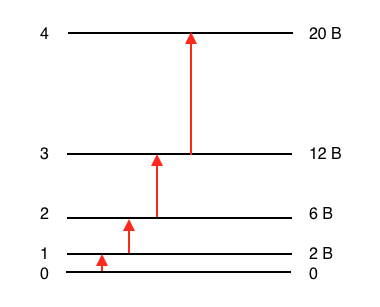
\includegraphics[width=0.5\textwidth]{figures/Energy_levels}
\caption{Rotational energy levels. Values for $\mathcal{J}$ are given on the left and corresponding energy
  levels (in units of the rotational constant $B$) are given on the right.}
\label{fig:energy_levels}
\end{center}
\end{figure}

This is an example of a \textbf{selection rule}. A closer look at the
red arrows in Figure \ref{fig:energy_levels} reveals that the allowed
transition energy differences are equidistant. They can be described
by the simple formula
\begin{equation}
\Delta E_\mathcal{J} = 2B(\mathcal{J}+1), \qquad \mathcal{J} = 0, 1, 2, ...\,.
\end{equation}

Besides their native unit of Joule,
energy(diferences) can be conveniently expressed in
\textbf{wavenumbers} (Kaysers)
\begin{equation}
\tilde{\nu} = \frac{\Delta E}{hc} \qquad \left[\frac{1}{cm}\right]
\end{equation}
or in frequency (Hz)
\begin{equation}
\nu = \frac{\Delta E}{h} \qquad \left[Hz\right] \quad ,
\end{equation}
so energy differences translate directly to the observed spectrum.

In the literature, molecular energy differences and the rotational
constant $B$ are most often given in
units of Kaysers.

Note that we have assumed in all the above that there is only one
axis around which the molecule can rotate. If there are more axis of
rotation, the spectrum will be more complex.

In the exercise, we will look at some of these rotational spectra.


\clearpage
% CHAPTER 3 - VIBRATIONAL SPECTRA
\section{Vibrational spectra}
Now we will turn to vibration, another mode of molecular internal
energy. Just like rotational energy, vibrational energy is quantified,
hence can lead to spectroscopic transitions (= absorption lines). I
will use the terms \emph{vibration} and \emph{oscillation} as synonyms here.

\subsection{Classical harmonic oscillator}
We start off by looking at a harmonic oscillator in classical
mechanics (see Figure \ref{Vibration_parabol}). We can picture a
diatomic molecule as two atoms (point masses), connected by a
spring. The simplest possible assumption on the restoring force $f$, if
the molecule is stretched or compressed, is 
\begin{equation}
\label{eq:hooke}
f = -k (r-r_{eq}) \qquad (\text{Hooke's law})
\end{equation}
at the point $r$ from the equilibrium point $r_{eq}$ with a spring
constant $k$. 

\begin{figure}
\begin{center}
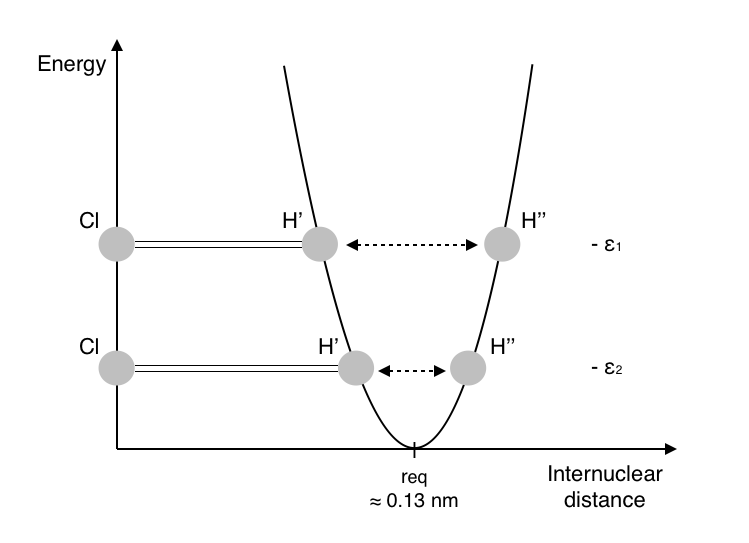
\includegraphics[width=0.9\textwidth]{figures/Vibration_parabol}
\caption{Energy curve for HCl molecules for extension or compression. After Banwell and McCash.}
\label{Vibration_parabol}
\end{center}
\end{figure}

Classically, if the molecule is stretched or squeezed a bit, it will
start to oscillate, due to the restoring force. The motion with this
particular restoring force is called \emph{harmonic oscillation} an is
described by sinusoidal functions. The angular frequency $\tilde{\omega}$ of the
oscillation is given by
\begin{equation}
\tilde{\omega} = \sqrt{\frac{k}{\mu}} \quad ,
\end{equation}
where $k$ is the spring constant from Equation \ref{eq:hooke} and
$\mu$ is the reduced mass, as defined in Equation
\ref{eq:def_mu}. (For a single `mass on a spring' pendulum, $\mu$
would simply be the mass, but for the system of two oscillating masses
we have to use the reduced mass.)

The essence of the equation above is that a stiffer spring leads to a
faster oscillation, whereas a larger (reduced) mass leads to a slower
oscillation. Both agrees well with intuition.

The energy that is contained in the vibration will depend on the
oscillation amplitude $\Delta r_{\mathrm{max}} = \max(r-r_{eq})$. At
the turning points (most stretched or compressed positions), there is
only potential (=spring) energy, and no kinetic energy. Because of
energy conservation, the total energy of the vibration stays on this
same value, only for example then the oscillation goes through
$r=r_{eq}$, all is in the form of kinetic energy. So, we can calculate
the energy contained in the vibration as
\begin{equation}
E = \frac{1}{2}k (r-r_{eq})^2 = \frac{1}{2} k {\Delta r}^2 \quad .
\end{equation}


\subsection{Quantum mechanical harmonic oscillator} 
For a real molecule, vibrational energy is quantised, so only certain
vibrational energy levels are allowed. The quantum mechanically possible energy levels turn out to be 
\begin{equation}
E_\nu = (\nu+\frac{1}{2})\hbar\tilde{\omega} \qquad (\nu = 0, 1, 2, ...) \quad ,
\end{equation}
where $\tilde{\omega} = 2 \pi \tilde{\nu}$ is the angular frequency of
vibration ($\tilde{\nu}$ being the plain frequency), and $\hbar =
h/(2\pi)$ is the reduced Planck constant (also called Dirac constant).

Transformed into spectroscopic units of Kayser we get
\begin{equation}
\epsilon_\nu = \frac{E_\nu}{hc} = (\nu + \frac{1}{2})\tilde{\nu} \qquad (\nu = 0, 1, 2, ...) \quad .
\end{equation}

The lowest vibrational level is at
\begin{equation}
E_0 = \frac{1}{2} \hbar \tilde{\omega} \quad .
\end{equation}
Therefore a molecule can never have \textbf{zero} vibrational energy!
This is different from rotation, where the lowest state had zero
energy. Figure \ref{Vibration_parabol_2} illustrates the vibrational
energy levels. Compare it to Figure \ref{fig:energy_levels} of the
rotational energy levels to see the fundamental difference: The
vibrational levels are equidistant.

\begin{figure}
\begin{center}
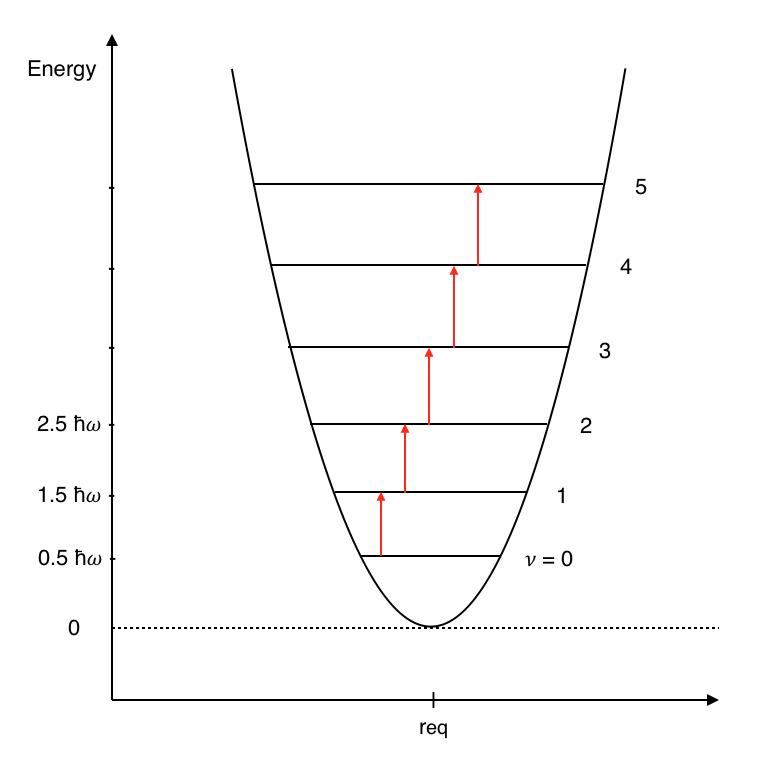
\includegraphics[width=0.7\textwidth]{figures/Vibration_parabol_2}
\caption{Allowed vibrational energy levels and transitions between them. After Banwell and McCash.}
\label{Vibration_parabol_2}
\end{center}
\end{figure}

The frequency of the observed spectral line corresponds to the energy
difference $\tilde{\nu}$ between adjacent levels. Since all the levels
are equidistant, all the possible `pure' vibrational transitions would
map to a single spectral line at frequency $\tilde{\nu}$. Put
typically such `pure' transitions are not allowed, only transitions
that also involve changes in the rotational state.

If molecules rotate, the energy separation is 1 - 10\,cm$^{-1}$
whereas if they vibrate, the energy separation is 100 -
10\,000\,cm$^{-1}$. This is a large difference in characteristic
energy. We can therefore assume that the two motions occur
independently.  (This is a case of the Born- Oppenheimer
approximation, which strictly also includes optical transitions). We
write
 \begin{gather}
E_{total} = E_{rot} + E_{vib} \qquad \left[J\right]  \\
\epsilon_{total} = \epsilon_{rot} + \epsilon_{vib} \qquad \left[cm^{-1}\right].
 \end{gather}
Combining the discrete energy levels results in
\begin{equation}
\epsilon_{\mathcal{J},\nu} = \epsilon_{\mathcal{J}} + \epsilon_{\nu} =
B \mathcal{J} (\mathcal{J} + 1) + (\nu + \frac{1}{2})\tilde{\nu} \quad .
\end{equation}
Note: There are higher order therms in both rotation (zentrifugal stretching) and vibration (non-constant restoring force) that I am ignoring here. \par
 
 \begin{figure}
\begin{center}
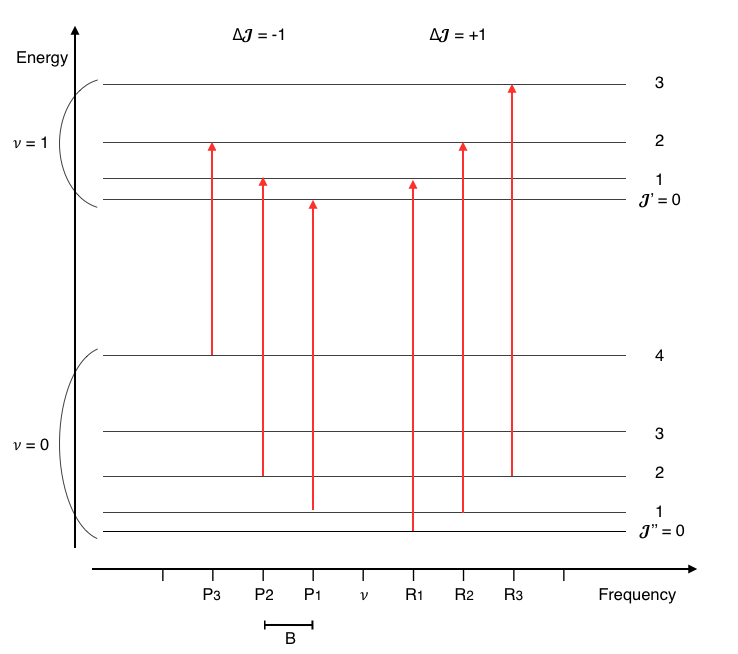
\includegraphics[width=0.75\textwidth]{figures/Transitions_vib_rot}
\caption{Transitons between vibrational - rotational energy levels. After Banwell and McCash.}
\label{Transitions_vib_rot}
\end{center}
\end{figure}
 
The selection rule states, that
\begin{equation}
\Delta \nu = 0,\pm 1 \quad \mathrm{and} \quad \Delta \mathcal{J} = \pm 1
\quad \text{(see Figure \ref{Transitions_vib_rot})} \quad .
\end{equation}
This means, we normally cannot observe the vibrational fundamental
directly. Rotational levels will be filled to varying degrees in a
population of molecules. This results in different line intensities. 

The transition frequencies are divided into two branches:
\begin{gather*}
\Delta \mathcal{J} = +1 \quad (\text{R-Branch}) \\
\qquad \Delta \epsilon_{\mathcal{J},\nu} = \tilde{\nu} + 2 B ( \mathcal{J''} + 1), 
	\qquad \mathcal{J''} = 0, 1, 2  \\
\Delta \mathcal{J} = -1 \quad (\text{P-Branch}) \\
\qquad \Delta \epsilon_{\mathcal{J},\nu} = \tilde{\nu} - 2 B ( \mathcal{J'} + 1) , 
	\qquad \mathcal{J'} = 0, 1, 2  \\ 
\end{gather*}
 They can be combined into: 
 \begin{equation}
\Delta \epsilon_{\mathcal{J},\nu} = \tilde{\nu} + 2 B m , 
	\qquad m = \pm1, \pm2, \pm3, ...
\end{equation}
These are the frequencies of the observed lines. 

So why are the branches called 'P' and 'R'? For more complicated molecules, $\Delta \mathcal{J} = 0 \text{ and } \pm 2$ may also be allowed. All possible branches are:


\begin{center}
\begin{tabular}{|c|c|c|c|c|c|} \hline
$\Delta\mathcal{J}$ = & -2 & -1 & 0 & +1 & +2 \\
\hline
Name & O & P & Q & R & S \\
\hline
\end{tabular}
\end{center}

The number of vibrational modes (different types of vibrations) in a
molecule is 3N-5 for linear molecules and 3N-6 for nonlinear
molecules, where N is the number of atoms (see for example
\url{http://www.wag.caltech.edu/home/jang/genchem/infrared.htm}). So,
for a diatomic molecule, there is only one possible mode of vibration,
just like there is only one mode of rotation.

More interesting are molecules with three or more atoms. The most
important molecules for Earth's greenhouse effect, 
H$_2$O and CO$_2$, are tri-atomic. There vibrational modes are
summarised in Figure \ref{fig:vib_modes}. H$_2$O is nonlinear, therefore it has
\begin{equation}
  n_\mathrm{vib,H2O} = 3*3-6 = 9-6 = 3
\end{equation}
vibrational modes. CO$_2$ is linear, therefore it has
\begin{equation}
  n_\mathrm{vib,CO2} = 3*3-5 = 9-5 = 4
\end{equation}
vibrational modes. However, two of these 4 modes (symmetric bending)
have the same fundamental frequency. One corresponds to motion in the
paper plain, as shown in Figure \ref{fig:vib_modes}, the other to
motion perpendicular to the paper plain. Furthermore, the symmetric
stretch mode of CO$_2$ at 1330 cm$^{-1}$ is not associated with a
change in the dipole moment, and therefore is not infrared active, so
that CO$_2$ has only two active infrared vibration modes.

\begin{figure}
\begin{center}
\begin{tabular}{| c | c | c | }
  \hline
  Symmetric stretch & Symmetric bend & Asymmetric stretch  \\
  \hline
  % H2O
\schemestart
\chemfig{@{a1}H-[:30,0.8]@{a2}O-[:-30,0.8]@{a3}H}
\arrow(@a1.south west--.south west){->}[210,0.6,line width=.4pt,blue]
\arrow(@a2.north--.north){->}[90,0.6,line width=.4pt,blue]
\arrow(@a3.south east--.north east){->}[-30,0.6,line width=.4pt,blue]
\schemestop &
\schemestart
\chemfig{@{a1}H-[:30,0.8]@{a2}O-[:-30,0.8]@{a3}H}
\arrow(@a1.north--.north){->}[90,0.6,line width=.4pt,blue]
\arrow(@a2.south--.south){->}[-90,0.6,line width=.4pt,blue]
\arrow(@a3.north--.north){->}[90,0.6,line width=.4pt,blue]
\schemestop &
\schemestart
\chemfig{@{a1}H-[:30,0.8]@{a2}O-[:-30,0.8]@{a3}H}
\arrow(@a1.south west--.south west){->}[210,0.6,line width=.4pt,blue]
\arrow(@a2.north east--.east){->}[0,0.6,line width=.4pt,blue]
\arrow(@a3.north east--.north west){->}[145,0.6,line width=.4pt,blue]
\schemestop  \\
  $\tilde{\nu}_1 = 3651.7 \text{\,cm}^{-1}$ &
  $\tilde{\nu}_2 = 1595.0 \text{\,cm}^{-1}$ &
  $\tilde{\nu}_3 = 3755.8 \text{\,cm}^{-1}$ \\
  \hline
  %CO2
\schemestart
\chemfig{@{a1}O-[,0.8]@{a2}C-[,0.8]@{a3}O}
\arrow(@a1.west--.west){->}[180,0.6,line width=.4pt,blue]
\arrow(@a3.east--.east){->}[0,0.6,line width=.4pt,blue]
\schemestop &
\schemestart
\chemfig{@{a1}O-[,0.8]@{a2}C-[,0.8]@{a3}O}
\arrow(@a1.north--.north){->}[90,0.6,line width=.4pt,blue]
\arrow(@a2.south--.south){->}[270,0.6,line width=.4pt,blue]
\arrow(@a3.north--.south){->}[90,0.6,line width=.4pt,blue]
\schemestop &
\schemestart
\chemfig{@{a1}O-[,0.8]@{a2}C-[,0.8]@{a3}O}
\arrow(@a1.north west--.north){->}[0,0.6,line width=.4pt,blue]
\arrow(@a2.south east--.south){->}[180,0.6,line width=.4pt,blue]
\arrow(@a3.east--.east){->}[0,0.6,line width=.4pt,blue]
\schemestop \\
  $\tilde{\nu}_1 = 1330.0 \text{\,cm}^{-1}$ &
  $\tilde{\nu}_2 = 667.3 \text{\,cm}^{-1}$ &
  $\tilde{\nu}_3 = 2349.3 \text{\,cm}^{-1}$ \\
\hline  
\end{tabular}
\end{center}
\caption{Vibrational modes of H$_2$O and CO$_2$.}
\label{fig:vib_modes}
\end{figure}



% CHAPTER 4 - LINE SHAPE
\section{Line shape}
\label{sec:line_shape}

There are three mechanisms that lead to a broadening of absorption lines:
\begin{itemize}
\item Natural line width
\item Pressure broadening
\item Doppler broadening 
\end{itemize}

\subsection{Natural line width}

So far we know that the difference between two energy states $E_{f}$
and $E_{i}$ equals the frequency $\nu$ times the Planck constant $h$:
\begin{equation}
h \nu = E_f - E_i \quad .
\end{equation}

So absorption (and emission) would happen at exactly one frequency and
the line shape would be a delta-function. There is a fundamental
quantum mechanical principle that prevents this from being true:
Heisenbergs's uncertainty principle sais that one cannot know position
and momentum of a particle simultaneously:
\begin{equation}
\Delta x \Delta p \approx \hbar \quad ,
\end{equation}
where $\hbar$ is the reduced Planck constant. Another manifestation of this principle is:
\begin{equation}
\Delta E \Delta t \approx \hbar = 10^{-34}~J s \quad .
\end{equation}

Thus, the shorter the lifetime of a state, the more uncertain is its energy. 
The groundstate has an infinite lifetime, so its energy is exactly known:
\begin{equation}
\Delta t = \infty \rightarrow \Delta E = 0 \quad .
\end{equation}

The first excited electronic state, however, has a finite lifetime
\begin{equation}
\Delta t = 10^{-8}~s \rightarrow \Delta E = \frac{\hbar}{\Delta t} =
\frac{10^{-34}}{10^{-8}} = 10^{-26}~J \quad ,
\end{equation}
and the associated frequency uncertainty is
\begin{equation}
\Delta \nu = \frac{\Delta E}{h} = \frac{10^{-26}~J}{10^{-34}~Js} =
10^{8}~Hz \quad .
\end{equation}

This seems a large number at first sight, but electronic transitions
typically have frequencies of $10^{14}$-$10^{16}$~Hz (visible spectral
range). Therefore natural line width can be considered as
small. However, the actual shape of the line is important.

The finite lifetime of the upper state means that it decays with time:
\begin{equation}
\frac{dn(t)}{dt} = -A n(t) \quad ,
\end{equation}
where $n$ is the number of molecules in the excited state and A is the
Einstein A coefficient for spontaneous emission. The solution of this
equation is
\begin{equation}
n(t) = n(0) e^{-At} = n(0) e^{-\frac{t}{\tau}} \quad ,
\end{equation}
where $\tau$ is the lifetime. 

The derivative $\frac{dn(t)}{dt}$ is the rate at which
the excited state decays, but at the same time it is also the rate of
spontaneously emitted photons (whenever a state decays, a photon is
emitted). Thus, for the radiation flux L we can write:
\begin{equation}
\label{eq:decay}
L(t) = L(0) e^{-At} \quad .
\end{equation}

So L also decays exponentially in time. If a signal amplitude is not
constant in time, it cannot be monochromatic. The frequency spectrum
is given by the Fourier transform of Equation \ref{eq:decay}:

\begin{equation}
F_{L}(\nu) = \frac{1}{\pi} \frac{A/4\pi}{(\nu - \nu_{0})^{2} +
  (A/4\pi)^{2}} = \frac{1}{\pi} \frac{\gamma_{N}}{(\nu - \nu_{0})^{2}
  + \gamma_{N}^{2}} \quad .
\end{equation}

$F_{L}$ is called a Lorentz-Function (also Cauchy distribution or
Breit Wigner distribution), and $\gamma_{N}$ is the natural line width parameter. 

\subsection{Doppler Broadening}

Doppler Broadening is conceptually simpler than natural broadening. It
is due to the thermal motion of the molecules, which Doppler-shifts
the frequency (at any point in time one part of the molecules is
moving towards me and one part is moving away). The
Maxwell-distribution for velocity (valid for LTE) is:

\begin{equation}
p(u) = \sqrt{\frac{m}{2\pi kT}} \,\, \exp \left(\frac{-mu^{2}}{2kT}
\right)  \quad ,
\end{equation}
where $u$ is the velocity and $m$ is the mass of the molecule. 
Non-relativistic Doppler-shift is given by
\begin{equation}
\nu - \nu_{0} = \frac{\nu_{0}u}{c} \quad .
\end{equation}

The faster the molecule, the larger the Doppler-shift. Combining this
with the Maxwell velocity distribution gives
\begin{equation}
F_{D}(\nu) = \frac{1}{\gamma_{D}\sqrt{\pi}} \,\, exp \left[- \left( \frac{\nu
    - \nu_{0}}{\gamma_{D}} \right )^{2} \right] \quad ,
\end{equation}
with the `Doppler width'
\begin{equation}
  \gamma_{D} = \frac{\nu}{c} \sqrt{\frac{2kT}{m}} \quad .
\end{equation}
Note that $F_{D}$ is a Gaussian.  

\subsection{Pressure Broadening}

Collisions between molecules also limit the lifetime of energy states
("collisional broadening"). If one assumes that collisions themselves
take no time, that there is no interaction between collisions and that
collisions completely "reset" the state, then the resulting shape is
again Lorentzian:
\begin{equation}
F_{L}(\nu) = \frac{1}{\pi} \frac{\gamma_{C}}{(\nu - \nu_{0})^{2} +
  \gamma_{C}^{2}} \quad .
\end{equation}

The rate of collision is proportional to pressure. Empirically $\gamma_{C}$ is calculated as follows:
\begin{equation}
\gamma_{C} = p \cdot \mathrm{AGAM} \left( \frac{T_{ref}}{T} \right)^{\mathrm{NAIR}} \quad ,
\end{equation}
where AGAM and NAIR are in the spectral line catalogue. (In reality there are some more parameters.) 

So which of the broadening mechanisms do we use in reality? We neglect
natural broadening, but have to use thermal and collisional broadening
($\gamma_{D}$ and $\gamma_{C}$). The shape then is a convolution of
Lorentz and Gauss shape, called "Voigt-Function". There is no
analytical form of this function, only numerical approximations.

In the exercise you will find out which effect of broadening dominates when. 


% CHAPTER 5 - THERMAL RADIATION
\section{Thermal radiation}

We now want to look at the balance between Radiation and
Temperature. If an object receives more radiation, its temperature
rises. And a higher temperature results in a higher emission of
radiation. We first look at a black body that absorbs all incoming
radiation without any reflection. This is the case e.g. in a hollow
space. If the Temperature is kept constant, there will be a radiative
equilibrium between the walls and the radiation on the inside of the
hollow space. This radiative equilibrium is \textit{only} dependent on
the temperature, every other dependancy would be contradicting the
laws of Thermodynamics.

The relationship between temperature and radiation is described in
what now is known as \textit{Planck's law}:
\begin{equation}
I_{\nu} = B_{\nu}(T) = \frac{2h\nu^3}{c^2(e^{\frac{h\nu}{kT}}-1)}, 
               \hspace{3cm} B_{\lambda}(T) = \frac{2hc^2}{\lambda^5(e^{\frac{hc}{\lambda kT}}-1)} \quad ,
\end{equation}
where $I_\nu$ is the spectral radiance
[W\,m$^{-2}$\,sr$^{-1}$\,Hz$^{-1}$], B the Planck function, T the
temperature, h the Plack constant, $\nu$ the frequency, c the speed of
light, k the Boltzmann constant and $\lambda$ the wave length.
The low frequency approximation of Planck's law is the
Rayleigh-Jeans law, which was already known before Planck's law:
\begin{equation}
I_{\nu} = B_{\nu, RJ}(T) = \frac{2kT}{c^2}\nu^2  \quad .
\end{equation}

Wien's displacement law states that the black body radiation curve for different temperatures peaks at a frequency proportional to the temperature
\begin{equation}
\nu_{max} \propto T  \quad .
\end{equation}

When radiation meets a surface, it is either absorbed or
reflected. The absorption coefficient $\alpha$ therefore has values
between 0 and 1. A body that emits thermal radiation has an emissivity
coefficient $\epsilon$ between 0 and 1. An emissivity coefficient
$\epsilon$ = 0 means no radiation is emitted, a body with $\epsilon$ =
1 emits the same amount of radiation that a blackbody of the same
temperature would emit:
\begin{equation}
I_\nu = \epsilon(\nu)B_\nu(T)  \quad .
\end{equation}

Absorption and Emission have to balanced, otherwise this would be
contradicting the second law of Thermodynamics. \textit{Kirchhoff's
  law of thermal radiation} states that for all frequencies and angles
\begin{equation}
\epsilon(\vartheta,\varphi,\nu) = \alpha(\vartheta,\varphi,\nu) \quad .
\end{equation}

We now apply these rules to our climate system. The earth itself emits
radiation at the temperature of its surface. Due to the natural
greenhouse effect, the temperature at earth's surface is increased by
34\,K. This can be seen in Figure \ref{Buehler_et_al_OLR_spectra}
which shows the spectra of longwave radiation of the earth as seen
from space.

 \begin{figure}
\begin{center}
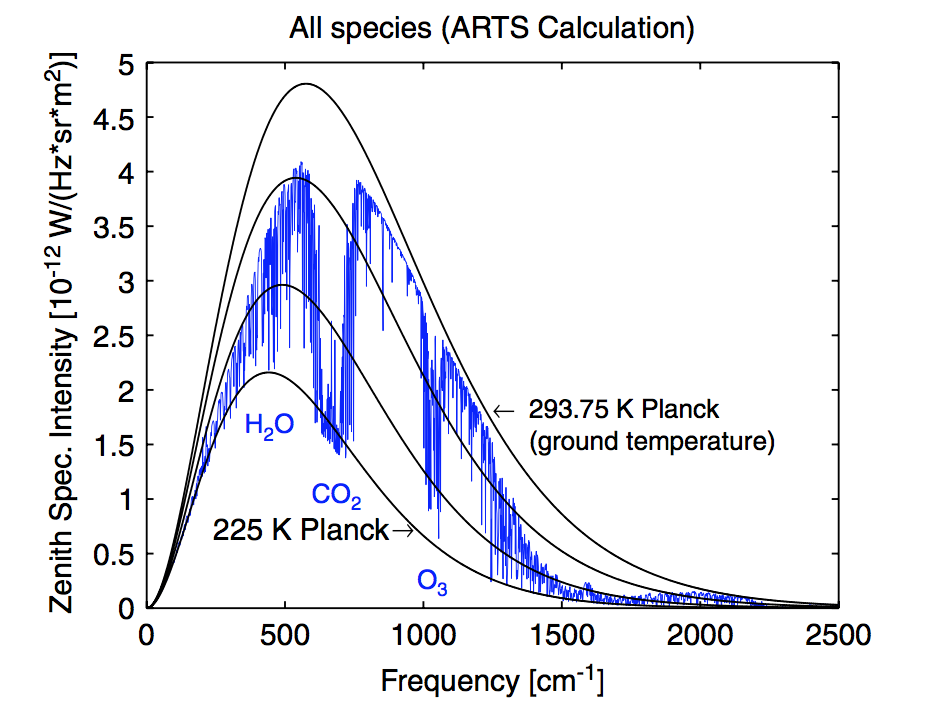
\includegraphics[width=0.85\textwidth]{figures/Buehler_et_al_OLR_spectra}
\caption{Clear-sky OLR spectra of the earth as seen from space. The area between the top curve and the blue curve is caused by the natural greenhouse effect. From Buehler et al., 2006.}
\label{Buehler_et_al_OLR_spectra}
\end{center}
\end{figure}

Comparing the radiational intensities to the Planck curves shows at
which temperature the radiation was emitted
\begin{equation}
T_b = B^{-1}_{\nu}(I_{\nu}) \quad ,
\end{equation}
where $T_b$ is called the brightness temperature. Using the brightness
temperature in remote sensing is very common since it is an intuitive
unit for the intensity. E.g., one would interpret $T_b = 300$\,K as a
high value since there are not much higher temperatures in the
atmosphere. $T_b = 200$\,K on the other hand, would not be very much.
 


% CHAPTER 6 - RADIATIVE TRANSFER EQUATION
\section{Radiative transfer equation}

First we need to define some important radiation quantities:
\begin{description}
\item[Spectral Radiance = monochromatic pencil beam radiance = Intensity ($I$)] The radiation power per square
  meter that is traveling in a particular direction, per frequency
  interval, per solid angle interval. Unit: 
  \begin{equation*}
    \frac{\mathrm{W}}{\mathrm{m^2  \, Hz \, sr}}
  \end{equation*}
\item[Radiance ($L$)] is obtained by integrating $I$ over frequency. Unit:
  \begin{equation*}
    \frac{\mathrm{W}}{\mathrm{m^2  \, sr}}
  \end{equation*}
\item[Irradiance = Radiative Flux ($F$)] is obtained by integrating $L$ over solid
  angle (one hemisphere), taking the projection onto the nominal
  direction of the flux. Unit:
  \begin{equation*}
    \frac{\mathrm{W}}{\mathrm{m^2}}
  \end{equation*}
\end{description}

The radiative transfer equation (RTE) describes the change of radiation along a path,
for example from the ground to a sensor above the surface. The RTE is expressed in 
terms of the Intensity $I$. It can be written as
\begin{equation}
	\frac{dI}{ds} = - (\alpha + \sigma)I + \alpha B(T) + \sigma \int_\Omega PI  \quad ,
	\frac{d\Omega}{4\pi}
\end{equation}
where $ds$ is a path element. The first term on the right hand side is 
the radiation loss due to extinction by absorption (absorption coefficient $\alpha$) 
and scattering (scattering coefficient $\sigma$). The second term is a source term
due to thermal emission $B(T)$. The third term is a source term due to radiation that
is scattered into the path. It is calculated using the phase matrix $P$ of the 
scattering particles. The calculation involves an integration of the intensity over the 
whole solid angle $\Omega$. Note, that normally every variable depends on the frequency
and the viewing direction. 

We see that if we include scattering in the RTE, it is very difficult to solve, because 
in order to compute the intensity in one direction, we need to know the intensity in 
every other direction.

One of the most used simplifications of the RTE is to neglect scattering. If we look at
thermal radiation, this is mostly true for a clear sky atmosphere. If we neglect 
scattering, the last term as well as the $\sigma$ in the first term vanish and the 
(clear sky) RTE looks like this:
\begin{equation}
	\frac{dI}{ds} = -\alpha I + \alpha B(T) = \alpha ( B(T) - I ) \quad .
\end{equation}
This equation is also known as Schwarzschild's equation because if was formulated by 
K. Schwarzschild in 1906. 

Using this equation, let's look at what happens in a homogeneous medium ($\alpha$ and $T$
constant). If the radiation passes through the medium long enough ($s \rightarrow \infty$)
the difference between $B$ and $I$ has to get smaller and smaller. This means that eventually,
$I$ will converge to $B$. This makes sense because if we look through a thick enough medium, 
we hardly see which radiation came into the medium, we only see the emission of the medium.\\
Schwarzschild's equation can be integrated along a path through a layer
(a complete derivation can be found in Petty, Eq. 8.5 - 8.13):
\begin{equation}
	I(s) = I(0) e^{-\tau (0,s)} + \int_{0}^{s} \alpha (s') B(s')  \quad ,
	e^{-\tau (s',s)} ds' 
\end{equation}
where $\tau(0,s)$ is the opacity between the points, defined as
\begin{equation}
	\tau (0,s) = \int_{0}^{s} \alpha(s') ds' \quad .
\end{equation}
We see that the layer emits radiation, while the incoming radiation $I(0)$ is 
attenuated exponentially. 

In radiative transfer models such as ARTS, the atmosphere is usually divided 
into homogeneous layers and the RTE is calculated through these layers. So to understand
the calculations in the model, it is useful to look at the solution of Schwarzschild's
equation in a homogeneous layer. The only difference is the opacity, which in a homogeneous
layer, we can write as
\begin{equation}
	\tau(0,s) = \int_{0}^{s} \alpha(s') ds' = \alpha s \quad .
\end{equation}

To get the solution, we just plug a homogeneous layer from 0 to $s$ into the integral 
form of the equation:
\begin{equation}
	I(s) = I(0) e^{-\alpha s} + \alpha B(T)\int_{0}^{s} e^{-\alpha (s-s')} ds'  \quad ,
\end{equation}
which, after some algebra, gives
\begin{equation}
	I(s) = I(0) e^{-\alpha s} + B(T) \left( 1-e^{-\alpha s}
        \right) \quad .
\end{equation}

With the definition of the transmission $t = e^{-\alpha s}$, we can rewrite the solution as
\begin{equation}
	I(s) = t I(0)  + \left( 1-t \right) B(T) \quad .
\end{equation}

It is instructional to look at two extreme cases of the solution:

\begin{description}
\item[Optically thick]
What happens if the opacity of the layer is very high, so $ t\rightarrow0$ ? 
Then we just see the Planck emission of the layer. The incoming radiation does not reach us.
\item[Optically thin]
What happens if the opacity of the layer is 0, to $ t \rightarrow 1$ ? Then we just see
the incoming radiation $I(0)$. The layer doesn't do anything.\\

A more interesting special case is when the opacity is small, but not zero. For small opacities, 
we can use a linear approximation of the transmission, which comes from the Taylor expansion
of the exponential function:
\begin{equation}
	t = e^{-\tau} \approx 1 - \tau \quad .
\end{equation}
If we plug this into the solution of a homogeneous layer, we get
\begin{equation}
	I(s) = t I(0)  + \left( 1-t \right) B(T) \approx I(0) + \tau \left( B - I(0)\right) \quad ,
\end{equation}
which has exactly the same form as Schwarzschild's equation itself.
\end{description}


% CHAPTER 7 - JACOBIANS
\section{Jacobians}
Inverse modeling is needed for estimating an atmospheric state variable
$\vec{x}$ by measuring an affected variable $\vec{y}$
\begin{equation*}
\vec{y}=F(\vec{x}) \rightarrow \vec{x}=?
\end{equation*}
The physical relationship between $\vec{x}$ and $\vec{y}$ is described by F, the
so called forward model:

\begin{equation*}
\vec{y}=F(\vec{x})+\vec{\epsilon} \quad ,
\end{equation*}
where $\vec{y}$ is the variable which should be measured,$F$ is the forward
model dependent on the variable of the atmospheric state $\vec{x}$ (e.g.
temperature profile, altitude)  and $\vec{\epsilon}$ is the noise.\\

\subsection*{Definition}
\textbf{Jacobian}:
The Jacobian is defined as the partial derivative of the forward model at the
$i^{th}$ element of the vector $\vec{y}$ (e.g. $i^{th}$ frequency) to a
variation of the $j^{th}$ element of the atmospheric state vector (e.g.
altitude).
\begin{equation*}
J_{i,j}=\frac{\partial F_i}{\partial x_j}
\end{equation*}

For example if the temperature is retrieved, then the Jacobian describes how
the brightness temperature ($\vec{y}$) at a certain frequency changes when the
temperature ($\vec{x}$) at the $j^{th}$ level changes.
Hence a Jacobian could be understood as the sensibility of $\vec{y}$ at the
$i^{th}$ element if the $j^{th}$ element of $\vec{x}$ varies.\
There are two possible methods of calculating a Jacobian.

\subsection*{Pertubation Method}
This method is a 'naive' but always working method. It is quite
straightforward to implement and can be used where other methods
fail. The Jacobian is calculated by perturbing the state variable
$\vec{x}$ by a small disturbance $\vec{\Delta x}$. The Jacobian
corresponding to the state variable $\vec{x}$ can thus be calculated
as
\begin{equation}
J(i,j)=\frac{\partial y_i}{\partial x_j} \approx \frac{\Delta y_i}{\Delta x_j} =
\frac{F(\vec{x}+\vec{\Delta x_j})-F(\vec{x})}{\Delta x} \quad ,
\end{equation}
where $\Delta x$ is the $j^{th}$ element of $\vec{\Delta x} $, as in:
{\setstretch{0.7}
	\begin{equation*}
	\vec{\Delta x}_j=\left[\begin{array}{c} 0 \\ \vdots \\0\\ \Delta x \\ 0\\ \vdots
	\\0\end{array}\right] \qquad
	\end{equation*}
}

This method is relatively inefficient because one has to run the full forward
model F for every element of $\vec{x}$, only perturbing them once at a time.

\subsection*{Analytical Method}
For the analytical method, we use the integral form of the clear-sky radiative
transfer equation (RTE) for a given frequency
\begin{equation*}
y=I=I_0 \cdot e^{-\int_0^\infty \alpha(s') ds'}+ \int_0^\infty \alpha(s)B(T(s)))
\cdot e^{-\int_0^s \alpha(s')ds'} ds \quad ,
\end{equation*}
where $\alpha$ is the absorption coefficient and B is the thermal emission. Or
in a discrete form
\begin{equation*}
I=I_0 \cdot \underbrace{\vphantom{\frac{a}{b}}e^{-\sum_{j=0}^N \alpha_j \Delta
		s_j'}}_{\substack{Transmission}}+ \sum_{i=0}^N
\underbrace{\vphantom{\frac{a}{b}}\alpha_i \Delta s_i
	B(T_i)}_{\substack{Emission}} \cdot
\underbrace{\vphantom{\frac{a}{b}}e^{\overbrace{-\sum_{j=0}^i \alpha_j \Delta
			s_j}^{Opacity}}}_{\substack{Transmission}} \quad ,
\end{equation*}
with the layerthickness $\Delta s$ and the incoming Radiation $I_0$.\\

As is shown in figure \ref{fig:perturbedLayer}, if the atmosphere is perturbed
at one layer, this will affect the emission at this layer and the transmission
of everything behind.
\begin{figure}
	\centering
	
	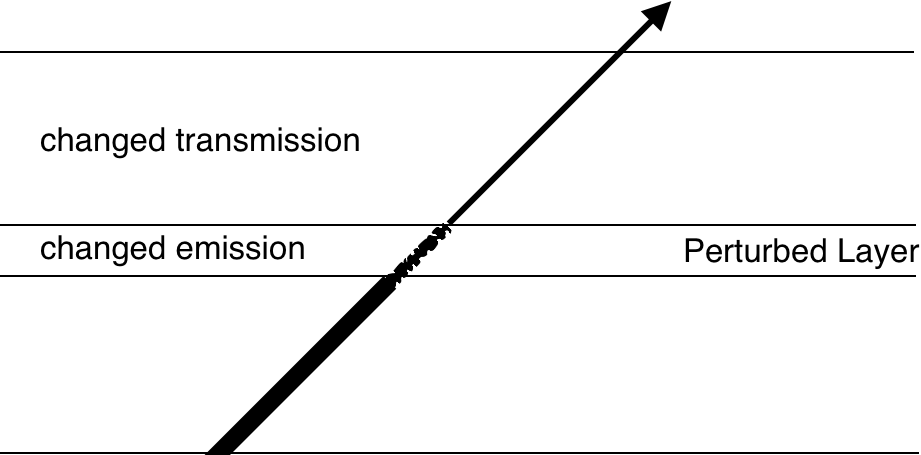
\includegraphics[width=0.6\textwidth]{./figures/perturbedLayer_EmissionTransmission}
	\caption{}
	\label{fig:perturbedLayer}
\end{figure}
\\
\textbf{Emission:}\\
\begin{equation*}
\frac{\partial}{\partial x_k}(\alpha_k \Delta s_k B(T_k)) = \Delta s_k B(T_k)
\frac{\partial \alpha_k}{\partial x_k}
\end{equation*}
If x is the number density of some gas(n):
\begin{equation}
\alpha=n \cdot \sigma \rightarrow \frac{\partial \alpha}{\partial
  n}=\sigma \quad ,
\end{equation}
where n is the density and $\sigma$ is the absorption cross-section.

\textbf{Transmission:}
\begin{equation}
\tau=\sum_{i=0}^N \alpha_i \Delta s_i = \alpha_1 \Delta s_1 + \alpha_2 \Delta
s_2 + \cdots + \alpha_N \Delta s_N \quad ,
\end{equation}
The change of the transmission can be written as
\begin{equation*}
\frac{\partial \tau}{\partial x_k}=\Delta s_k \frac{\partial \alpha_k}{\partial
	x_k} \quad .
\end{equation*}

\subsection*{Pro and Cons of the different calculations of Jacobians}
\textbf{Numerical Perturbation Method}
This method is very easy to implement and it works for any parameter in a
"black-box" kind of way which makes the method very "foolproof". Therefore it
takes a lot of time to calculate the Jacobian.
\\\\
\textbf{Analytical Method}
This method needs a lot of "housekeeping" and is not always feasible. But it is
also more accurate and faster than the Numerical Perturbation Method.

\subsection*{Displaying Jacobians}
Since the Jacobian is a matrix, there are three basic ways to display it:\\
1. \textbf{Contour plot:} Frequency dependence for all altitudes, figure
\ref{fig:plotTypes}a)\\
2. \textbf{Row plot:} Altitude dependence for selected frequencies, figure
\ref{fig:plotTypes}b)\\
3. \textbf{Column plot:} Frequency dependence for selected altitudes, figure
\ref{fig:plotTypes}c)

\begin{figure}
	\centering
	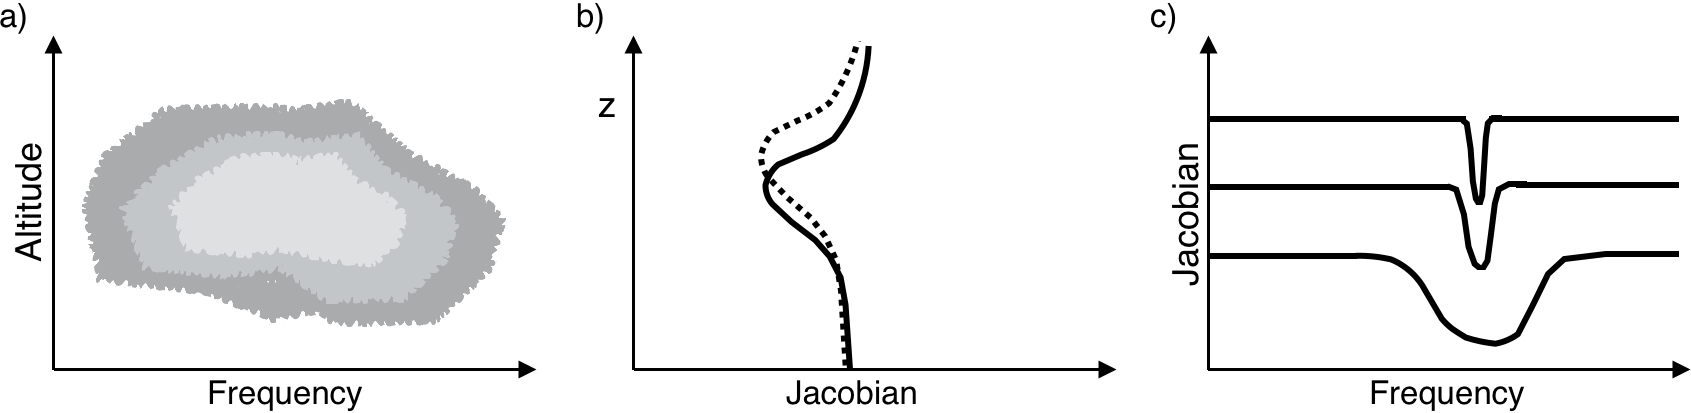
\includegraphics[width=\textwidth]{./figures/plotTypes_Jacobian}
	\caption{}
	\label{fig:plotTypes}
\end{figure}

\subsection*{Opacity rule}
Jacobians tell us where the information comes from or rather where changes in
the atmosphere affect the radiation most.\\
The opacity rule tells us something about the origin of the radiation. The
origin of the thermal radiation is the distance where the opacity, as calculated
from the observer, reaches 1.
\end{document}

%%% Local Variables:
%%% mode: latex
%%% TeX-master: "AdvRaRe_script_print"
%%% End:
